In this section, we present experimental results to study the performance
of our model in the task of complex action recognition. Our experimental
validation focuses on measuring two aspects of our model.
First, we measure action classification accuracy on
several action recognition benchmarks.
Second, we validate the performance of our model at the
task of spatio-temporal atomic action
annotation of human body regions that are involved in performing the complex
action.

%This section described the experimental results in heterogeneous datasets. We
%first describes each dataset to specify the experimental setup, whith a brief
%explanation of why we choose each dataset to evaluate our model. Later, we
%focus in the strenght of our model, in producing rich annotations in addition
%to the semantic global labels. 

%\subsection{Experimental Setup}
In the following experiments, we evaluate our method on four action recognition
benchmarks:
the MSR-Action3D dataset \cite{WanLi2010},
Concurrent Actions dataset \cite{Wei2013},
Composable Activities Dataset \cite{Lillo2014}, and sub-JHMDB
\cite{Jhuang2013}.


\subsection{Classification of Simple and Isolated Actions}

As a first experiment,
we evaluate the performance of our model on the task of simple and
isolated human action recognition in the  MSR-Action3D dataset
\cite{WanLi2010}.
Note that although our model is tailored at recognition of complex human
actions, this experiment verifies the performance of our model in the
simpler scenario of isolated atomic action classification.

The MSR-Action3D dataset provides depth videos and estimated body poses
for isolated actors in pre-trimmed videos performing actions from 20
categories. We use 557 videos in the dataset in a similar setup to
\cite{Wang2012}, where videos from subjects 1, 3, 5, 7, 9 are used for
training and the rest for testing.

We measure action classification accuracy and report the results obtained
by our model and other competing methods in Table \ref{tab:msr3d}.
We note that our model achieves comparable performance with respect
to the state-of-the-art methods for simple action recognition.

\begin{table}[t]
\footnotesize
\centering
\begin{tabular}{|l|c|}
\hline
\textbf{Algorithm} & \textbf{Accuracy}\\
\hline
Our model &  93.0\% \\
%Ours, GEO+VEL, NI &  93.0\% \\
%Ours, GEO+VEL  & 91.2\% \\
\hline
L. Tao \etal \cite{Tao2015} & 93.6\% \\
C. Wang \etal \cite{Wang2013} &    90.2\% \\
Vemulapalli \etal \cite{Vemulapalli2014} & 89.5\% \\
%Lillo et al. \cite{Lillo2014} & 89.5\%\\
\hline
\end{tabular}
\caption{\footnotesize
Action classification performances in the MSR-Action3D dataset. }
\vspace{-4mm}
\label{tab:msr3d}
\end{table}

%\paragraph{MSR-Action3D} Setup: subjects 1,3,5,7,9 for training, rest for
%testing, using all 20 action categories. This dataset is more as a proof of
%concept, that our model achieves near state-of-the-art accuracy in a standard
%dataset.
%In fact, omitting Tao el at. ICCV 2015 paper, we would achieve the
%best accuracy. BUT, they do not provide the rich annotations for testing data
%as our model. Also, we use the same initialization method to automatically
%annotate the actions in the dataset: the initialization method is integrated
%with the model and is independent of the dataset.

%\paragraph{MSR-Action3D} A very popular skeleton + Depth single action dataset.
%We use the common setup of using skeleton data from
%, using all 20 action categories. We
%use 557 videos from the dataset as proposed by \cite{Wang2012}. We use this
%dataset to show how our model performs in a standard database of single
%actions.


\subsection{Detection of Concurrent Actions}
Our second experiment evaluates the performance of our model in a concurrent
action recognition setting. In this scenario, the goal is to predict
the temporal localization of actions that may occur concurrently in a long
video.

We evaluate this task on the Concurrent Actions dataset \cite{Wei2013},
which
provides 61 RGBD videos and pose estimation data annotated with 12
action categories of interest.
We use a similar evaluation setup as proposed by the authors.
We split the dataset into training and testing sets with a 50\%-50\% ratio.
We evaluate performance by measuring precision-recall: a detected action
is declared as a true positive if its temporal overlap with the ground
truth action interval is larger than 60\% of ther union, or if
the detected interval is completely covered by the ground truth annotation.

Our model is tailored at recognizing complex actions that are composed
of atomic components. However, in this scenario, only atomic actions are
provided and no compositions are explicitly defined. We therefore apply
a simple preprocessing step: we cluster training videos into groups
by comparing the occurrence of atomic actions within each video.
The resulting groupings are used as complex actions labels in the training
videos of this dataset.

Note that at inference time, our model outputs a single labeling per video,
which corresponds to the atomic action labeling that maximizes the energy of
our model.
Since there are no thresholds to adjust, our model produces a single
precision-recall measurement as reported in Table \ref{tab:concurrent}.
We observe that our model outperforms the state-of-the-art method in this
dataset at that recall level.


%\paragraph{Concurrent Action dataset} This dataset has 61 videos of variable
%time, some of them are very long comoared to other action datasets. The videos
%has a variable number of actions. The skeleton data and action annotations are
%provided in the dataset.
%We select randomly 50\% of videos for training and the
%rest for testing.

%We want to show using this dataset that the latent formulation achieve good
%recognition performance with respect to the model that uses this dataset. We
%can show also new annotations in this dataset, corresponding to the regions
%that are annotated with the actions.


\begin{table}[tb]
\footnotesize
\centering
\begin{tabular}{|l|c|c|}
\hline
\textbf{Algorithm} & \textbf{Precision} & \textbf{Recall}\\
\hline
%Ours, GEO+VEL, NI, VL-KM-ST &  92.3\% & 0.81\% \\
Our model &  0.92 & 0.81 \\
\hline
Wei et al. \cite{Wei2013} & 0.85 & 0.81 \\
\hline
\end{tabular}
\caption{
\footnotesize
Action detection performances in the Concurrent Actions dataset. }
\label{tab:concurrent}
\vspace{-3mm}
\end{table}
 
\subsection{Recognition of Composable Activities}
In this experiment, we study the performance of our model in terms of
classification of complex and composable actions.
For this purpose, we use the Composable Activities dataset \cite{Lillo2014},
which provides 693 videos of 14 subjects performing 16 composable activities.
Each activity is formed as a spatio-temporal composition of atomic actions.
The dataset provides a total of 26 atomic actions that are shared across
activities.

Table \ref{tab:composable} summarizes our experimental results.
We report activity recognition accuracy for two versions of our
model: one trained with spatial supervision that indicates which
body regions are involved in each action, and another with
no spatial supervision where no body regions are annotated and $V$
is treated as a latent variable.
We observe that both models achieve comparable performance, which
indicates that our weakly supervised model can recover some of the information
that is missing and still perform well at the activity catergorization task.
It is also interesting to note that in spite of using less
supervision at training time, our method outperforms the state-of-the-art
methodologies that are trained with full spatial supervision.
% of the body parts
%and regions that are involved in each atomic actions.


\begin{table}[tb]
\footnotesize
\centering
\begin{tabular}{|l|c|}
\hline
\textbf{Algorithm} & \textbf{Accuracy}\\
\hline
Our model, with spatial supervision &  91.8\% \\
Our model, no spatial supervision ($V$ Latent) & 91.1\%\\
%Ours, GEO+TRAJ &  91.1\% \\
%Ours, GEO+TRAJ, NI  & 91.8\% \\
%Ours, GEO+TRAJ, NI, VL-KM-ST   & 91.1\% \\
\hline
%J. Luo et al. \cite{luo2013group} & \textbf{96.7\%} \\
%Y. Zhu et al. \cite{zhu2013fusing} & 94.3\% \\
Lillo \etal \cite{Lillo2014} & 85.7\% \\
%BoW & 74.1\%    \\
%HMM & 78.9\%  \\
Cao et al. \cite{cao2015spatio} & 79.0\% \\
%H-BoW & 82.4\%   \\
%2-lev-HIER & 83.8\%  \\
\hline
\end{tabular}
\caption{
\footnotesize
Human action classification performances in the Composable Activities
dataset.}
\vspace{-4mm}
\label{tab:composable}
\end{table}
 
\subsection{Action Recognition in RGB Videos}
Our experiments so far have evaluated the performance of our model
in the task of human action recognition in RGBD videos.
In this experiment, we explore the use of our model in the problem of human
action recognition in RGB videos. For this purpose, we use the sub-JHMDB
dataset \cite{Jhuang2013}, which focuses on videos depicting 12 actions and
where most of the actor body pose is visible in the image frames.
In our validation, we use the 2D body pose configurations provided by the
authors and compare performance against previous methods that also use them.
We summarize the results of this experiment in Table \ref{tab:subjhmdb},
which shows that our method outperforms alternative action recognition algorithms
in the state-of-the-art.

%\paragraph{sub-JHMDB} In this dataset, we use the annotated joints provided to
%build our geometric descriptor. Only 15 joints per frame are annotated, and the
%coordinates of the joins are in 2D image coordinates.
%We first translate the
%15 joints into 20 joints, and also create a \emph{pseudo} 3D data by adding a
%$z=0$ coordinate to the joints, adding $d$ to the joints of wrists and knees,
%and subtracting $d$ for elbows, to create a 3D skeleton suitable to our model.
%AS RGB videos are available, we compute the TRAJ feature as in Composble
%Acivities Dataset (explain better).

%For a fair
%comparison, we compare our method with works that used the ground truth joints.
%We show in the results the mean accuracy over three splits, provided in the
%dataset.

\begin{table}[tb]
\footnotesize
\centering
\begin{tabular}{|l|c|}
\hline
\textbf{Algorithm} & \textbf{Accuracy}\\
\hline
Our model &  77.5\% \\
\hline
Huang et al. \cite{Jhuang2013} & 75.6\% \\
Ch\'eron et al. \cite{Cheron2015} & 72.5\%\\
\hline
\end{tabular}
\caption{\footnotesize
Action classification performances in the sub-JHMDB dataset.}
\label{tab:subjhmdb}
\vspace{-4mm}
\end{table}


\subsection{Spatio-temporal Annotation of Atomic Actions}
In this experiment, we study the ability of our model to spatially annotate
actions.
Table \ref{tab:annotation} summarizes our annotation performance
results.
After training our model, we measure precision-recall for the spatio-temporal
atomic action annotations predicted by our model in the testing videos
(first row).
This is a very challenging task, as
the testing videos are not provided any labels and the model
should predict the temporal extent of each action and the regions of the
body associated with it. We note that our model achieves good performance
in this annotation task.

Furthermore, we also study the capability of the model in annotating
the spatial body region during training. In this case, each video is provided
with the temporal extent of actions and only the spatial anotation needs to
be inferred (second row).
Finally, we note that if we run the trained model over the training videos
without providing any labels (third row), the model is still able to
spatio-temporally annotate atomic actions with performance similar to the
one obtained for the testing set.
%Note that this is due to the fact
%that we are not directly optimizing for atomic action annotation
%We also analyze the performance of the model in discovering the true atomic
%action annotations in the training set.
%our model.


\begin{table}[tb]
\footnotesize
\centering
\begin{tabular}{|l|c|c|c|}
\hline
\textbf{Videos} & \textbf{Annotation} & \textbf{Precision} & \textbf{Recall}\\
\hline
Testing set & Spatio-temporal   & 0.62 & 0.78 \\
\hline
Training set & Spatial only & 0.86 & 0.90\\
Training set & Spatio-temporal & 0.67 & 0.85 \\
\hline
\end{tabular}
\caption{
\footnotesize
Atomic action annotation performances in the Composable Activities
dataset. The results show that our model is able to recover spatio-temporal
annotations both at training and testing time.}
\label{tab:annotation}
\vspace{-3mm}
\end{table}


\subsection{Effect of Model Components}
In this experiment,
we study the contribution in terms of performance of each component of the
model.
We focus our validation on the Composable Activities dataset for the purpose
of this experiment.

Table \ref{tab:components} summarizes our experimental results with different
versions of our model. We focus on three main components of our model:
the garbage collector for poses (GC), Actionlets, and no spatial supervision
on body regions ($V$ Latent).
Our reported results in Table \ref{tab:components} show that the full version
of our model achieves the best performance, with each component contributing
to the overall success of the method.

%In this dataset is clear tee benefits of all the components of the model: as we
%only have a single action label per video, we use the initialization of videos
%to get a better representation of the actions in the videos.
%As this dataset is
%from videos \emph{on the wild}, the camera view varies from video to video,
%making this dataset specially suitable to our algorithm of multiple classifiers
%per semantic action. Finally, the same as the rest of datasets, including the
%garbage collector math in the model allows to get a more discriminative model
%as it feeds the pose classifiers only with most informative poses.


\begin{table}[tb]
\footnotesize
\centering
\begin{tabular}{|l|c|}
\hline
\textbf{Algorithm} & \textbf{Accuracy}\\
\hline
Base Model & 70.6\%\\
Base Model + GC & 72.7\% \\
Base Model + Actionlets & 75.3\%\\
Our full model (Actionlets + GC + $V$ Latent) &  77.5\% \\
\hline
\end{tabular}
\caption{
\footnotesize
Analysis of contribution to recognition performance from
each model component in the sub-JHMDB dataset.}
\label{tab:components}
\vspace{-4mm}
\end{table}

We also analize the contribution of our self-paced learning framework
for intializing and training our model.
As in any discriminative model with latent variables, initialization
is important.
We summarize our results in
Table \ref{tab:initialization} by reporting action
recogntion accuracy obtained by the model under different initialization schemes.
We compare our initialization method to two baselines. First,
we initialize the latent variables $V$ randomly. Second, we initialize $V$ by
performing clustering on region descriptors.
We note that our initialization method help the model to achieve its best
performance.

\begin{table}[tb]
\footnotesize
\centering
\begin{tabular}{|l|c|}
\hline
\textbf{Initialization Algorithm} & \textbf{Accuracy}\\
\hline
Random   & 46.3\% \\
Clustering   & 54.8\% \\
Ours   & 91.1\% \\
\hline
\end{tabular}
\caption{
\footnotesize
Results in Composable Activities dataset, using V latent, showing different initializations. }
\label{tab:initialization}
\vspace{-3mm}
\end{table}

\subsection{Qualitative Results}

\begin{figure}[th]
\begin{center}
%\fbox{\rule{0pt}{2in} \rule{0.9\linewidth}{0pt}}
%\includegraphics[width=0.9\linewidth]{./Fig/poselets.pdf}
\scriptsize
 Motion poselet \#4 - most probable action: talking on cellphone\\
 \includegraphics[trim=0 0 0 0.35cm, clip, width=0.49\textwidth]{Fig/poselets1}

 Motion poselet \#7 - most probable action: erasing on board\\
 \includegraphics[trim=0 0 0 0.35cm, clip, width=0.49\textwidth]{Fig/poselets2}

 Motion poselet \#19 - most probable action: waving hand\\
 \includegraphics[trim=0 0 0 0.35cm, clip, width=0.49\textwidth]{Fig/poselets3}
\end{center}
\caption{TBD}
\label{fig:poselets_img}
\end{figure}


\begin{figure}[th]
\begin{center}
\scriptsize
 Motion poselet \#16 - most probable action: tennis swing\\
 \includegraphics[trim=0 0 5.5cm 0.25cm, clip, width=0.49\textwidth]{Fig/poselets4}

 Motion poselet \#34 - most probable action: golf swing\\
 \includegraphics[trim=0 0 5.5cm 0.25cm,clip, width=0.49\textwidth]{Fig/poselets5}

 Motion poselet \#160 - most probable action: bend\\
 \includegraphics[trim=0 0 5.5cm 0.25cm, clip, width=0.49\textwidth]{Fig/poselets6}


\end{center}
\caption{TBD}
\label{fig:poselets_skel}
\end{figure}


\begin{comment}

[GENERAL IDEA]

What we want to show:
\begin{itemize}
\item Show tables of results that can be useful to compare the model.
\item Show how the model is useful for videos of simple and composed actions, since now the level of annotations is similar.
\item Show how the inference produces annotated data (poses, actions, etc). In particular, show in Composable Activities and Concurrent actions how the action compositions are handled by the model without post-processing.
\item Show results in sub-JHMDB,showing how the model detects the action in the videos and also which part of the body performs the action (search for well-behaved videos). It could be interesting to show the annotated data over real RGB videos. 
\item Show examples of poses (like poselets) and sequences of 3 or 5 poses for actions (Actionlets?)
\end{itemize}

\subsection{Figures}
The list of figures should include:
\begin{itemize}
\item A figure showing the recognition and mid-level labels of Composable Activities, using RGB videos
\item Comparison of action annotations, real v/s inferred in training set, showing we can recover (almost) the original annotations.
\item Show a figure similar to Concurrent Actions paper, with a timeline showing the actions in color. We can show that our inference is more stable than proposed in that paper, and it is visually more similar to the ground truth than the other methods.
\item Show a figure for sub-JHMDB dataset, where we can detect temporally and spatially the action without annotations in the training set.
\item Show Composable Activities and sub-JHMDB  the most representative poses and actions.
\end{itemize}


\paragraph{Composable Activities Dataset}
In this dataset we show several results.
(1) Comparing TRAJ descriptor (HOF over trajectory);
(2) Compare the results using latent variables for action assignations to
regions, with different initializations;
(3) Show results of the annotations of the videos in inference.

We must include figures comparing the real annotations
and the inferred annotations for training data, to show we are able to get the
annotations only from data.



%%We report results on two publicly available datasets:
%the MSR-Action3D \cite{WanLi2010} dataset for benchmarking recognition of simple actions,
%and our Composable Activities Dataset introduced in \cite{Lillo2014}.
%We next describe each dataset as well as some implementation details.

While our model is aimed at the recognition of activities that can be composed by simpler actions,
we experimentally verify that the model can also handle the case of simple action recognition.
Towards this goal, we evaluate our algorithm on the MSR-Action3D dataset \cite{WanLi2010},
which consists of 10 subjects performing 20 actions related to gaming in front of a TV.
This dataset provides skeleton data (joint locations) and low resolution depth maps.

During training, our hierarchical model needs 
a global activity label as well as per-frame atomic action labels. However, the MSR-Action3D 
dataset only includes the annotation of a single global action for each video. As a consequence, 
we need to augment the annotations of this dataset to be compatible with our model. To achieve 
this, we automatically augment the annotations as follows. At the activity level of our model, we 
use the original action label provided in the dataset as our global activity
label. Similarly, at the atomic action level of our model, 
we annotate each video frame with this global action label. As a further adaptation, we swap to an
\emph{idle} label all inactive frames. We select the frames annotated as \emph{idle} following a 
simple heuristic. First, we annotate as 
\emph{idle} the four body regions of the first frame of each video. Then, we search for all frames 
in which the pose of each region closely resembles the corresponding pose in
the first frame, labeling all these regions as \emph{idle} too. This simple heuristic works well to 
identify \emph{idle}
frames in this dataset, since subjects start the video
with a resting position. Additionally, we filter out noisy \emph{idle} labels by 
only keeping as such sets of more than 6 consecutives frames labeled as \emph{idle}. Finally, 
we assign a complete region in a video as \emph{idle} if this label appears in more than 60\% of 
the 
frames.

In our experiments, we use a total of 552 sequences.
We omit 5 out of the 557 videos because they have missing joints in
the last half of the sequence.
We test our model on all 20 action categories using cross-subject validation,
with subjects 1-3-5-7-9 for training and the rest for testing.
This corresponds to the same experimental setting used in \cite{Wang2012}.
In our evaluation, we use $K=100$ poses for each body region, for a total of 400 pose 
dictionary entries.

%%%%%%%%%%%%%%%%%%%%%%%%%%%%%%%%%%%%%%
\begin{table}
\centering
%{\small
\begin{tabular}{|c|c|}
\hline
\textbf{Algorithm} & \textbf{Accuracy}\\
\hline
Ours  &  \textbf{92.4\%} \\
\hline
%J. Luo et al. \cite{luo2013group} & \textbf{96.7\%} \\
%Y. Zhu et al. \cite{zhu2013fusing} & 94.3\% \\
C. Wang et al.\cite{Wang2013} &    90.2\% \\
Vemulapalli et al. \cite{vemulapalli2014human} & 89.5\% \\
Lillo et al. \cite{Lillo2014} & 89.5\%\\
Xia and Aggarwal \cite{Xia} & 89.3\% \\
J. Wang et al. \cite{Wang2012} &   88.2\% \\

\hline
\end{tabular}
%}
\caption{Recognition accuracy of our approach in the MSR-Action3D dataset compared to other
methods in the literature that also use the experimental setup in 
\cite{Wang2012}. Our method improves state-of-the-art
performance in this dataset.
%We include methods that use
%joint data only and evaluation using cross-subject using all 20 action categories.
}
%\vspace{-0.3cm}
\label{tab:msr_st}
\end{table}
%%%%%%%%%%%%%%%%%%%%%%%%%%%%%%%%%%%5
Table \ref{tab:msr_st} reports the overall recognition accuracy of our model
in the MSR-Action3D dataset,
as measured by the average of the diagonal of the normalized confusion matrix. Additionally,
Table \ref{tab:msr_st} compares our results to alternative methods proposed in the literature
that also use the training/testing setup proposed in \cite{Wang2012}.
Under this experimental setting, our model improves the state-of-art accuracy
in this dataset.

%\JC{Alvaro: queda cojo pues finalmente solo se reporta el accuracy como todos
%los otros modelos. Hay que conectar esto con algun resultado cuantitativo o
%cualitativo que muestre las ventajas indicadas}
In addition to the strong activity recognition performance, our model
has also the advantage of generating a rich video interpretation in the form of
detailed per-frame and per-body-region action annotations.
In contrast, all competitive models only produce a coarse interpretation
in the form of a global video label prediction. Section \ref{subsec:action_annotation} provides 
quantitative and qualitative insights about the capabilities of our method to infer at each frame 
the body regions executing the action.

An important aspect of these results is that our model achieves
this performance using a pose dictionary of only 100 entries per region.
This compares favorably with the results reported in \cite{Wang2012}, \cite{Wang2013}, and 
\cite{Xia},
which use dictionaries with thousands of entries.
Our reduced dictionary translates to more compact models that require
less computation at the inference stage. 

%Furthermore, our model does not require a previous 
%temporal segmentation as \cite{Koppula2012} or \cite{Wei2013}, the 
%inputs to our model are only the frame descriptors.

%As we will see in Section \ref{subsec:sparse_reg}, using a larger pose dictionary does not produce 
%necessarily better results in our model, as well as a huge increasing in $K$ will make the 
%inference impractical since the computing time is proportional to $K^2$.


%%%%%%%%%%%%%%%%%%%%%%%%%%%%%%%%%%%5
\begin{table}
\centering
%{\small
\begin{tabular}{|c|c|c|c|}
\hline
\textbf{Algorithm} & \textbf{GEO} & \textbf{GEO/MOV} & \textbf{GEO/MOV + NI} \\
\hline
Ours, QR  &  89.5\% & 90.6\% & \textbf{92.4\%} \\
\hline
\end{tabular}
%}
\caption{Recognition accuracy of our approach in MSR-Action3D using a quadratic regularizer 
(QR) and different settings: i) Using only a geometric 
descriptor (GEO), ii) Combining  a geometric and a motion descriptors (GEO/MOV), and iii) Adding a 
mechanism to identify and discard non-informative poses (NI).}
%\vspace{-0.3cm}
\label{tab:msr}
\end{table}
%%%%%%%%%%%%%%%%%%%%%%%%%%%%%%%%%%%%%

%\JC{Alvaro: mover a mas adelante, donde se explican los efectos indicados,
%i.e., secciones 4.3 y 4.4.}
Finally, Table \ref{tab:msr} reports the performance of our model
under several settings. First, we report performance when
the model uses a quadratic regularizer (QR)
combined with the geometric descriptor described in Section 
\ref{subsec:videorepresentation} (GEO). This corresponds to the setup used in 
\cite{Lillo2014}. We also consider the case when we combine the geometric descriptor with the 
motion 
descriptor described in Section 
\ref{subsec:videorepresentation} (GEO/MOV). Additionally, we consider the case when the model 
includes the 
proposed method to identify and discard non-informative (NI).
We further discuss the effect of these settings in the following sections.

%We report the overall recognition accuracy as measured by the average of the
%diagonal of the normalized confusion matrix.
%We specify in the experiments when the 
%quadratic regularizer (\textbf{QR})
%or sparse regularizer (\textbf{SR}) is applied, as well as if the descriptor
%used is only geometric (\textbf{GEO}), or a fused descriptor including geometry
%and motion (\textbf{GEO/MOV}). We also specify when the handling of
%non-informative poses is applied (\textbf{NI}).

% Here we explain the databases, give implementation details, and all the extra info needed to understand the following sections.
\subsection{Recognition of composable activities}
\label{subsec:experiments_summary}
%In order to test the suitability of our model for recognition of complex and
composable activities, we use
the Composable Activities benchmark dataset from \cite{Lillo2014}.
This dataset consists of 694 RGB-D
videos that contain activities in 16 classes performed by 14 actors. Each
RGB-D sequence is captured using a Microsoft Kinect sensor, with the
position of relevant body joints estimated using \cite{Microsoft2012}.
Each activity in this dataset is spatio-temporally
composed by a variable number of mid-level (atomic) actions. The total number of
actions in the videos is 25 (plus an \emph{idle} action), while the number of actions
that compose each particular activity fluctuates between 2 to 10 actions.
For instance, the activity \emph{Walking while waving hand} has a spatio-temporal
composition of 2 single actions: \emph{walking} and \emph{waving hand};
while the activity \emph{Composed activity 4} is composed of 10 single actions:
 \emph{walking}, \emph{calling with hands}, \emph{waving hand},
\emph{talking on cellphone}, \emph{picking from floor}, \emph{throwing an object},
\emph{putting an object}, \emph{picking cellphone from pocket}, and \emph{putting
cellphone into pocket}, see Fig. \ref{fig:frontfigure} for some examples.
Every actor performs each activity 3 times in average.
Fig. \ref{fig_activities_actions_table} summarizes the composition of actions for
each activity.
The RGB-D data and annotations for this dataset are publicly available on
our project webpage\footnote{\url{http://web.ing.puc.cl/~ialillo/sparse_hier_activities}}.
%
\begin{figure}[tb]
\begin{center}
\includegraphics[width=0.999\linewidth]{./fig_activities_actions_table.pdf}
\end{center}
\caption{Composition of actions (columns) into activities (rows). Note that some activities are simpler, composed only by two actions, while others are very complex, including up to ten different atomic actions per video. Activities also share an \emph{idle} action, not shown in the table.}
\label{fig_activities_actions_table}
\end{figure}
%

Recognition rates for the Composable Activities Dataset are summarized in Table
\ref{Table-UniNorte}. 
We report performance averaged over multiple runs
using a leave-one-subject-out cross-validation strategy.
We use a validation set to experimentally adjust the value of all the main
parameters.
In practice, we set $\lambda_1 = 100$ and $\lambda_2 = 20$.
We set $K=50$ pose dictionary entries per body region when using the quadratic
regularizer (QR), and $K=150$ per body region when using the sparse
regularizer (SR).
We also reduce the temporal resolution for faster processing by
a factor of 6,
so the effective frame rate for all videos in training and recognition is 5 fps.

\begin{table}
\centering
{\small
\begin{tabular}{|c|c|c|}
\hline
\textbf{Algorithm} & \textbf{GEO} &  \textbf{GEO/MOV}  \\
\hline
Ours, SR+NI& $-$  &  \textbf{92.2\%} \\
Ours, QR+NI& $-$  & 91.8\%  \\
Ours, SR& 84.9\%  & 90.6\%  \\
Ours, QR& 85.7\%  & 90.9\%   \\
\hline
BoW& 67.2\% & 74.1\%    \\
HMM& 76.5\% & 78.9\%  \\
H-BoW& 74.2\% & 82.4\%   \\
2-lev-HIER& 79.6\% & 83.8\%  \\
\hline
LG \cite{vemulapalli2014human} & 74.7\% & $-$  \\
\hline
\end{tabular}
}
\normalsize
\caption{Recognition accuracy of our method compared to several baselines (see text in Section
\ref{subsec:exp_setup}). It is noteworthy that our 3-level model outperforms all 2-levels models. 
Also, as seen in the accuracy for our model, including motion cues in the descriptor (GEO/MOV) and 
using non-informative poses handling (NI) improve the accuracy over our previous model. The best 
performance is obtained when using all the contributions described in this work.
%\JC{JC: Convertir la ultima columna a dos filas: QR + NI, SR + NI}}
}
\label{Table-UniNorte}
%\vspace{-0.4cm}
\end{table}

The confusion matrix obtained with our full model is reported in
Fig.~\ref{fig:confusion_activities}. Note that for some activities the
prediction is perfect, while for others there is high confusion between
some activities, indicating probably highly similar poses like
\emph{calling with hands} and \emph{waving hand}, where many actors
perform the \emph{calling with hands} action with only one arm.

\begin{figure}[tb]
\begin{center}
\includegraphics[width=0.999\linewidth]{./conf_matrix.pdf}
\end{center}
   \caption{Confusion matrix for the activity classification task in the Composable Activities 
dataset, using sparse regularization, a fused descriptor and NI handling.}
\label{fig:confusion_activities}
\end{figure}

To show the semantic interpretation of the poses learned by our model, Fig. 
\ref{fig:example_poses_by_activity} shows top-scoring frames for three activities executed by 
different 
subjects. In general, our model produces highly interpretable poses that are 
associated to characteristic body configurations of the underlying atomic actions. To further 
illustrate this observation, Fig. \ref{fig:poses} shows the highest activations for eight pose 
dictionary entries associated to the body region corresponding to the left arm. In each case, 
Fig. \ref{fig:poses} also indicates the atomic action that assigns a greatest relevance (weight) to 
the corresponding pose. 
%\JC{Alvaro: No entiendo bien la ultima frase. Ademas, uno de los revisores pidio mostrar figuras de las poses aprendidas por el metodo. Podemos unir con esto?. Quizas mostrando con algun color el area de la pose identificada. O ejemplos caracteristicos de las poses, como en el paper de Bourdev and Malik sobre poselets (ECCV, 2012).}

\begin{figure}[tb]
\begin{center}
\includegraphics[width=0.999\linewidth]{./fig_examples_poses_by_activity.pdf}
\end{center}
   \caption{Examples of top score frames for three activities. Note the high correlation between the actions that compose each activity and the pose of the actors.}
\label{fig:example_poses_by_activity}
\end{figure}


\begin{figure}[tb]
\begin{center}
\includegraphics[width=0.999\linewidth]{./fig_poses.pdf}
\end{center}
   \caption{Examples of top scored poses for the body 
region corresponding to the left arm. Also shown, it is the label of the action with 
the highest classifier weight associated to the pose. In this case the model is trained using SR 
and $K=150$ for 
each body region.}
\label{fig:poses}
\end{figure}

As shown in Table \ref{Table-UniNorte}, we place our recognition results in context by comparing 
them to the performance of
two baselines methods, two simplified versions of our model, and a state-of-the-art algorithm.
The first baseline is based on a bag of words framework
(BoW), which only captures very coarse per-region
pose orderings and uses an independently pre-trained pose dictionary. Specifically, 
this baseline uses $k$-means to quantize pose descriptors
for each body region independently, which are aggregated into
a temporal pyramid histogram representation.
This is then fed into a multi-class linear SVM
for directly mapping from video descriptors to activities. 
The accuracy of this
baseline is 74.1\% when using the combined
descriptor based on geometric and motion information.

As a second baseline, we implement a Hidden Markov Model (HMM).
The HMM model can directly encode pose and action transitions built
upon an independently pre-trained pose dictionary.
In our implementation, states are trained with supervision by assigning one
state to each atomic action. Quantized poses are the observed variables.
We train models independently for each class, and at testing time,
we classify new sequences by assigning the label that corresponds to the
highest scoring model. The accuracy of this
baseline is 78.9\% when using the combined
descriptor based on geometric and motion information. While the ordering encoded by the HMM model 
helps to improve accuracy over BoW,
it still lacks the discriminative power of the top layer in our model for
jointly learning model parameters for all classes. 


We also compare performance against two simplified versions of our hierarchical
model. The first simplified version (H-BoW) does not jointly
learn the pose dictionary, but uses a fixed pose quantization obtained with
$k$-means, and omits the transition terms.
Unlike our full model, this simplified version does not take advantage of
jointly learning the pose dictionary, which leads to sub-optimal
pose encoding at the lower level of the hierarchy.
Also, by omitting the transition terms, the model cannot capture patterns
in the evolution of actions and poses.
These simplifications lead to a 10\% drop in performance in comparison
to our full model.

As a second simplification of our full model, we construct a
hierarchical model (2-lev-HIER) with two jointly learned
layers that encode poses and atomic actions. Activity recognition
is performed by an independently trained linear
classifier on top of the inferred atomic actions.
In this case, the performance of this model simplification is 8.4\% lower
than our full model. It is interesting that even when seemingly the top two
levels are uncoupled and one could train them independently,
there are benefits in jointly learning them.
%The action prediction in our 3-level hierarchical model is highly
%connected to the activity that is imputed during classification
%(recall that for classification we exhaustively search for each activity which
%produces the highest scored sequence of actions and poses, as
%Equation (\ref{eq:classify_inference})).
%Finally, jointly learning the pose dictionary is also beneficial, 
%as we gain about 3\% in accuracy when compared to
%using a pre-trained pose dictionary.


We also compare against an existing state-of-the-art algorithm from
the literature. In this case, we compare to the
method recently described in \cite{vemulapalli2014human} (LG).
%Another simple model is LG \cite{vemulapalli2014human},
We select this algorithm because it achieves state-of-art
performance on several pose-based action datasets. We train this model to
directly predict the activities from poses, omitting the mid-level
annotations, as in the BoW baseline. While the accuracy of LG is above BoW, it is
still 11\% lower than our model that only uses geometric information (GEO).

%\JC{General comments}:
%
%It is worth to note that all baselines that omit the mid-level
%(atomic actions) annotations (BoW and LG) perform worse that the the others
%that use that information.
%
%Our results confirm that jointly learning the
%classifiers in three levels (activities, actions and poses) outperform simpler
%setups by around 10\% of accuracy.


\subsection{Impact of including motion features}
\label{subsec:exp_motionfeats}

\subsection{Impact of latent spatial assignment of actions}
\label{subsec:exp_vlatent}
%In the preliminary version of our model \cite{Lillo2014},
we describe each frame using cues related to the geometry of the skeleton joints (GEO).
%we only use body joint positions from the estimated skeleton to compute our descriptor,
%disregarding valuable RGB motion information.
In this paper, we augment the representation by including a dynamic descriptor
that captures local dynamic information
as described in Section \ref{subsec:videorepresentation}. As reported in Tables \ref{tab:msr} and 
\ref{Table-UniNorte}, we present experimental results using the geometric descriptor (GEO), as well 
as the fused descriptor (GEO/MOV).

It is important to note that giving that the MSR-Action3D dataset does not include RGB information,
we modify the motion descriptor described in Section 
\ref{subsec:videorepresentation}. Specifically,
we encode differences of displacements for every joint, in a similar setup to
\cite{WangCVPR2011}.
This results in an 18 dimensional motion descriptor for each body region,
since each region contains 6 joints and each joint is a 3D vector.
The preliminary the version of our model \cite{Lillo2014} that uses
a quadratic regularizer and geometric features only,
we achieve a classification accuracy of 89.5\%.
By incorporating dynamic features,
we achieve an action classification accuracy of 90.6\%, reducing the error by 1.1\%. In the 
Composable Activities dataset, we use the motion descriptor described in Section 
\ref{subsec:videorepresentation}.
By adding the dynamic descriptor, the
improvement in accuracy is more notorious than in MSR-Action3D,
reducing the error by 5.2\% and 5.7\% according to the use of QR or SR regularizers, respectively.

Fig. \ref{fig:geo_mov_importance} shows the relative weight
of the geometric descriptor and motion descriptor in relation to each activity class
for the right arm and right leg. Focusing on right arm (left graph), note that
for actions like \emph{scratching head}, \emph{throwing an object} or
\emph{erasing the board}, the geometry of the joints is relatively more
important that the motion cues. Inversely, for other actions like
\emph{gesticulating} or \emph{calling with hands} the motion descriptor is more
important in average, since for these actions the movement of the arm is where
the information is encoded. 

\begin{figure}[tb]
\begin{center}
%\fbox{\rule{0pt}{2in} \rule{0.999\linewidth}{0pt}}
\includegraphics[height=2.2 in]{./fig_desc_relative_right_arm_mod.pdf}
\includegraphics[height=2.2 in]{./fig_desc_relative_right_leg_mod.pdf}
\end{center}
\caption{Relative importance of geometric (GEO) and motion (MOV) descriptors for right arm (left) and right leg (right).}
\label{fig:geo_mov_importance}
\end{figure}


\subsection{Impact of using multiple classifiers per semantic action}
\label{subsec:exp_multiple}
%%\JC{Alvaro: El primer parrafo repite la explicacion ya presentada en seccion 3.4.}
%In this paper, we have extended our model by introducing sparse
%regularization to improve the use of poses in the dictionary.
%In the preliminary version of our framework \cite{Lillo2014}, the model
%parameters are optimized using a quadratic regularization, leading to unregularized pose assignments.
In this paper we extend our preliminary model by introducing
a new regularizer that consists of a mixture of $L_2$ and $L_1$
norms for the atomic action
classifiers $\beta$ (see Equation \ref{eq:general_regularizer}).
The goal of the new regularization is to obtain a more
efficient use of the dictionary of body poses, in the sense that the model
learns more specialized poses for each atomic action, which also encourages
the fewer poses to be influential for each activity. For testing the effects of
sparse regularization in $\beta$, we use the Composable Activities dataset since
it provides richer hierarchical annotations.
We use fixed values $\mu=0.1$ and $\rho=5$ of
Eq. (\ref{eq:general_regularizer}) using sparse regularizer
(SR), contrasting the usual values used for $L_2$ regularizer (QR) $\mu=1$ and
$\rho=0$. Also, for QR setup, the number of poses is set to $K=50$ per body
region, while for SR is set to $K=150$ per body region.

In our experiments, we observe that when using SR only 8 to 11\% of the coefficients of $\beta$
remain non-zero. In average, this means a reduction of 85\% in the number of non-zero terms 
with respect to the use of QR. In terms of accuracy, as we see in Table \ref{Table-UniNorte},
recognition performance using sparse regularizer (SR) is similar to the case of
a quadratic
regularizer (QR), decreasing the error in 0.4\% when using the fused descriptor
and NI handling, and slightly increasing the error when the other modifications
are not applied. Despite the similar recognition accuracy provided by both regularizers, we 
identify at least three relevant advantages of using the SR setup:

\paragraph{i) Increased robustness to overfitting problems when using a sparse regularizer.} Figure 
\ref{fig:acc_vs_K_CA} shows recognition accuracy in function of the pose dictionary size $K$ when 
using QR and SR in
the Composable Activities dataset. We observe that when using QR the model clearly overfits as the 
dictionary grows larger than $K=50$. In contrast, using the SR setup, the
accuracy tends to increase or at least hold when larger dictionaries are used.
This behavior shows that the model using SR regularizer is best suited to be used
in larger models, since the learned poses are more specialized, and the model shows an 
increased robustness to overfitting problems. 

\begin{figure}[tb]
\begin{center}
%\fbox{\rule{0pt}{2in} \rule{0.999\linewidth}{0pt}}
\includegraphics[width=0.999\linewidth]{./fig_acc_vs_K.pdf}
\end{center}
\caption{Accuracy of testing versus the number of pose dictionary entries per
body region ($K$), for QR and SR setups. Note the decreasing accuracy of QR
setup (quadratic regularizer), indicating overfitting when more pose dictionary
elements are used, whereas using a sparse regularizer (SR) the accuracy remains
almost with no change. } \label{fig:acc_vs_K_CA}
\end{figure}

\paragraph{ii) Fewer poses influence each activity.}
One of the goals of using a sparse regularizer is to decrease the number of
entries from the pose dictionary that are used by each action classifier.
Since few pose dictionary entries
are required to explain each action (and therefore each activity),
this encourages every action to rely on a smaller group of poses, which usually
helps in improving the generalization power of the model,
the semantic interpretability of the poses,
and the efficiency of the pose dictionary.
%The
%influence (Eq. (\ref{XX})) of the poses aggregated for all activities
%and \ref{fig:poses_decay_C6}. Note the fast decay for pose influence when
%using the
%sparse regularizer, meaning that the model will focus on less poses when inferring the
%activity and actions of the video. Also, note the less decay in a more complex
%activity like \emph{Composed Activity 6} compared to \emph{Walking while hand waving};
%more poses influence the classification when the activity is more complex.
To illustrate this behavior, Figure \ref{fig:influence_agg} includes two diagrams corresponding to 
the influence (measured by Eq. (\ref{eq:influence})) of the
pose dictionary entries of right arm, across all activities, for QR setup (top
diagram) and SR setup (bottom diagram). We binarize the influence using a threshold
corresponding to the 5\% of the top influence value, to better showcase the
grouping effect.  For a fair comparison, $K=50$ is used in both setups, and we
use the same initial pose labels $Z$ to make the poses comparable. It is clear
from the figure that in the QR setup each activity is influenced by many poses
(and therefore each pose entry has activations in many activities), without a
clear pattern of pose activations. In this setup, 17.8 pose entries
influence each activity in average;
in contrast, for SR setup, only 8.6 poses in
average are influential for each activity, showing a sparse pattern. Since the
pose dictionary and atomic action classifiers are shared by all activities, the
grouping effect is straightforward, since the activities that share a common
action will also share its poses. As an example, if we observe the activations for the 
three activities
composed by the action \emph{Talking on cellphone}, many common poses are shared by these three
activities, and few of them are not, showing a grouping effect. Moreover, for those activities that 
do not
share atomic actions, the poses tend to be also non-shared. We omit from the
analysis the \emph{idle} action to enforce the influence of actual annotated
actions.

\begin{figure}[tb]
\begin{center}
%\fbox{\rule{0pt}{2in} \rule{0.999\linewidth}{0pt}}
\includegraphics[width=0.999\linewidth]{./fig_influence_QR_vs_SR.pdf}
\end{center}
\caption{Graphical representation of the influence of right-arm poses (using
$K=50$) in the activities of the Composable Activities dataset, using quadratic
regularizer (QR) and sparse regularizer (SR) (black is for influence score above a given 
threshold). Note that the SR setup
allows each activity to be represented by fewer poses, increasing the
interpretability of the poses generated by the model and the efficiency in pose
usage.
%\JC{JC: Aqui negro es desactivo, en la fig 9, negro indica activo. Es un poco confuso...}
%\JC{Alvaro: Seria posible generar una figura en que se cambia el orden del eje
%X. Tal que se ordena segun hamming distance (in a binary vector como cada
%columna de la figura), esto deberia permitir la visualizacion de grupos.
%Tambien se podria reportar el numero promedio de features usadas en figuras a
%y b para mostrar la reduccion del numero de poses usadas por cada clase.}
}
\label{fig:influence_agg}
\end{figure}
%
\paragraph{iii) Improved semantical interpretation of poses.}
The SR setup helps to improve the semantic meaning of the learned poses.
Observing Fig. \ref{fig:influence_agg}, the learned poses are
related to the actions involved in the activities. For example, just considering
poses 1 to 5 in the figure, we observe that in the SR setup they influence
the activities \emph{Composed Activity 4}, \emph{Waving hand and drinking}, and
\emph{Walking while waving hand}. It is clear that this 
group of poses correspond to the
right arm body region. Furthermore, they are related to the \emph{waiving hand} action, since 
it is the only
action that appears in all these activities. This kind of interpretation is not
possible under the QR setup. We foresee that the relevance of this type of interpretations can 
increase as new recognition scenarios will require the interpretation
of a larger number of actions. Note that we omit the \emph{idle} action when computing the influence scores for clarity (all activities share the\emph{idle} action), that is why some rows of Fig. \ref{fig:influence_agg} are all white (not influential to any activity).

%Additionally, we force the
%coefficients of the activity and atomic action classifiers to be positive, forcing the
%model to focus in the poses actually \emph{present} in each action and activity, and
%not \emph{punishing} the poses that should not be present. It is remarkable that using
%only positives weights for $\alpha$ and $\beta$, and also using small groups of poses
%for each $\beta$, the recognition accuracy is the same as the more unconstrained
%discriminative problem. We see several advantages in using the sparse regularizer with
%positive weights: the model does a more efficient use of the pose dictionary, as higher level
%classifiers only see relevant poses. By using only positives weights in the higher level
%classifiers, we are fostering the model to behave similarly to a generative model, so
%merging two activities to create a new composed activity could be made at no cost.
%%; we
%%will explore this property as part of our future work.
%Also, the positive weights
%force the model to focus on present actions in the videos, making the activity
%classifiers naturally sparse.



%\textforreview{
%In addition to the regulaizer, the extended model also adds a new term into
%the loss function that
%penalizes the diversity of learned poses inside an executed atomic action: for
%testing videos, the diversity of poses decreases 30\% compared to the previous
%model (QR), and 21\% compared to the new model using sparse regularizer but
%without considering the pose diversity penalty. All three models have similar
%accuracy on test videos, but the proposed sparse model produces each video to be
%represented by a small number of more representative learned poses.
%}


%\begin{figure*}[t]
%\begin{center}
%\includegraphics[width=0.95\linewidth]{./Influence_WH_modelGS_H.pdf} \\ (a) \\
%\includegraphics[width=0.95\linewidth]{./Influence_WH_model_H.pdf} \\ (b) \\
%\end{center}
%\caption{Influence of poses in activity \emph{Walk while calling with hands}. (a) using a sparse regularizer, (b) using a quadratic regularizer. The induced sparsity in the coefficients of action classifiers produces highly specialized poses. In this case, few poses are necessary to describe the arms (waving hand action), and more poses are needed to represent the walking action. Observing (a) we can speculate that most actors execute the \emph{waving hand} action using the right arm.}
%\label{fig:poses_decay_WH}
%%\vspace{-0.6cm}
%\end{figure*}
%
%\begin{figure*}[t]
%\begin{center}
%\includegraphics[width=0.95\linewidth]{./Influence_C6_modelGS_H.pdf} \\ (a) \\
%\includegraphics[width=0.95\linewidth]{./Influence_C6_model_H.pdf} \\ (b) \\
%\end{center}
%\caption{Influence of poses in activity \emph{Composed Activity 6}. (a) using a sparse regularizer, (b) using a quadratic regularizer. Comparing to Fig. \ref{fig:poses_decay_WH}, we can see that more poses influence this activity, which is expected since this activity is more complex than \emph{Walk while calling with hands}.}
%\label{fig:poses_decay_C6}
%%\vspace{-0.6cm}
%\end{figure*}


\subsection{Impact of handling non-informative poses}
\label{subsec:exp_non_info_handling}
%In our framework, we include a mechanism to identify and discard non-informative poses (NI) 
appearing in some frames. The mechanism assigns a learnable score $\theta$ to frame poses
that are non-informative to the action classifier
(see Eq. (\ref{Eq_poseEnergy})).
The poses from these frames are not accumulated into the pose histograms that
are fed to the action classifiers.
This enables to model to focus on more discriminative poses, which results in
more discriminative classifiers.

During learning, we need to initialize the set of candidate frame poses that can be considered 
as NI.
In practice, we initialize the NI poses by using the initial pose
dictionary obtained with $k$-means, and selecting as NI the poses that are
most distant to their assigned cluster centers. For each video,
we initially assign a total of 20\% of the frames to the NI bucket.
%To initialize training, during the first step of the learning algorithm the NI
%frames are assigned to be the 20\% of the most disperse frames, in terms of the
%distance to the assigned cluster center computed with $k$-means.
As the learning progresses, on each iteration poses can be reassigned to
a pose dictionary entry or to NI. In general, we observe that after convergence approximately 
17\% of all training frames are assigned as non-informative.
When we initialize the NI assignment with 40\% of the frames,
our final model reduces this to 19\%.
This indicates that
our model is effectively learning to detect non-informative frames in
the training videos.
%A similar behavior is observed when selecting 40\% of frames as initial
%non-informative frames, ending with 19\% of non-informative frames. This shows
%the dataset, and opens an entire field to test the same idea in, for example,
%patch-based object recognition.
%On the other hand,
%Also, 65\% of the initial NI poses were reassigned to a pose dictionary entry,
Moreover, near 40\% of the initial pose assignments are updated throughout
the iterations. This is compared to 25\% in preliminary model without
non-informative pose handling. This indicates that our full model is capable of
updating the pose representations more effectively.

In terms of accuracy, the use of NI reduces the error in 1.8\% in
MSR-Action3D, raising the accuracy from 90.6\% to 92.4\%. In the Composable Activities dataset the 
introduction of NI causes the error to
drop 1.4\% when using the SR regularizer, for a recognition accuracy of 92.2\%.
%

An important ability of the NI mechanism is that occluded regions are often
assigned as NI poses. Figure \ref{fig:non_info_poses_sequence} shows a
sequence of the activity \emph{Walking while reading}. In this figure, the bottom graph shows with 
black boxes frames where a body region is identified by our method as corresponding to a 
non-informative pose. Observing the body region corresponding to the arms, the long sequences of 
non-informative
poses nearly coincides with the occlusion periods of the arms (thick gray lines). Other frames
considered as non-informative tend to be sparser in time, and they can be
explained by rare poses or noisy body joints estimation. This behavior is
advantageous in two ways: during learning, it allows the model to
automatically disregard many occluded regions when learning the pose
classifiers; and during testing, it allows the model to identify possible occluded regions.

\begin{figure*}[t]
\begin{center}
\includegraphics[width=0.999\linewidth]{./fig_non_iinfo_poses.pdf}
\end{center}
\caption{\textforreview{Non-informative pose sequence for the four regions of
the body, in a video from the activity \emph{Walking while reading}. The black
squares represent frames labeled as a non-informative pose. A thick gray line
shows when the corresponding region is occluded. We can observe a relation between body region 
occlusions and identification of non-informative poses. Specifically,  when there is no occlusion, 
the identification of non-informative poses
tends to be temporally sparse, but for occluded intervals, many consecutive
frames are selected as non-informative.} } \label{fig:non_info_poses_sequence}
\end{figure*}

Figure \ref{fig:NI_handling} shows a comparison of some learned pose dictionary
entries with and without NI handling related to the activity \emph{Composed
Activity 5}, whose main atomic actions are \emph{walking},
\emph{gesticulating}, \emph{erasing board} and \emph{writing on board}. We show
the best-scored and worst-scored frames where two or more body regions are not
\emph{idle} or labeled as non-informative, i.e., correspond to poses that are
supposed to be discriminative for the activity.
Figure \ref{fig:NI_handling} illustrates that when using NI handling, the worst scored
frames imputed
as informative still preserve the semantics of the actions performed, while
without NI, the worst poses are noisy and without real meaning for the
performed action. Moreover, the non-informative frames in the right
clearly show poses that are not specific to the activity (or any activity),
and are correctly labeled as non-informative poses. This shows that using NI handling also helps 
to increase the semantic interpretation of the learned pose classifiers.

\begin{figure*}[tb]
\begin{center}
%\fbox{\rule{0pt}{2in} \rule{0.999\linewidth}{0pt}}
\includegraphics[width=0.999\linewidth]{./fig_NI_poses.pdf}
\end{center}
\caption{Comparison of frames showing poses from videos of the activity
\emph{Composed Activity 5}. All the presented frames belong to a subset of
frames where there is at least two body regions active for the underlying action
(not \emph{idle}). The best-scored
frames are similar with both setups. However, when considering the worse-scored
frames, it is clear that for the original model there are poses that are
not helping to the activity prediction. In general, those poses are labeled as
non-informative with our proposed modification, where the worse-scored poses of the new model
still remain discriminative and semantically valid for the target activity.}
\label{fig:NI_handling}
\end{figure*}

\end{comment}



%%%%%%%%%%%%%%%%%%%%%%%%%%%%%%%%%%%%%%%%%%%%%%%%555
%%%%%%%%%%%%%%%%%%%%%%%%%%%%%%%%%%%%%%%%%%%%%%%%%%
%
% COMMENTED SECTION FOR CAD120, INCLUDE IT SOMEWHERE IF THERE IS RESULTS IN
% THIS DATASET
%
%%%%%%%%%%%%%%%%%%%%%%%%%%%%%%%%%%%%%%%%%%%%%%%%%%
%%%%%%%%%%%%%%%%%%%%%%%%%%%%%%%%%%%%%%%%%%%%%%%%%%

\begin{comment}
\subsection{CAD120 Dataset}
The CAD120 dataset is introduced in \cite{Koppula2012}. It is composed of 124
videos that contain activities in 10 clases performed by 4 actors. Activities
are related to daily living: \emph{making cereal}, \emph{stacking objects}, or
\emph{taking a meal}. Each activity is composed of simpler actions like
\emph{reaching}, \emph{moving}, or \emph{eating}. In this database, human-object
interactions are an important cue to identify the actions, so object
locations and object affordances are provided as annotations. Performance
evaluation is made through leave-one-subject-out cross-validation. Given
that our method does not consider objects, we use only
the data corresponding to 3D joints of the skeletons. As shown in Table
\ref{Table-CAD120},
our method outperforms the results reported in
\cite{Koppula2012} using the same experimental setup. It is clear that using
only 3D joints is not enough to characterize each action or activity in this
dataset. As part of our future work, we expect that adding information related
to objects will further improve accuracy.
%
\begin{table}
\centering
{\small
\begin{tabular}{|c|c|c|}
\hline
\textbf{Algorithm} & \textbf{Average precision} & \textbf{Average recall}\\
\hline
Our method &  32.6\% & 34.58\% \\
\hline
\cite{Koppula2012} &   27.4\% & 31.2\%\\
\cite{Sung2012} &  23.7\%  &  23.7\% \\
\hline
\end{tabular}
}
\caption{Recognition accuracy of our method compared to state-of-the-art methods
using CAD120 dataset.}
\label{Table-CAD120}
\end{table}
\end{comment}
%
%%%%%%%%%%%%%%%%%%%%%%%%%%%%%%%%%%%%%%%%%%%%%%%%%%
%%%%%%%%%%%%%%%%%%%%%%%%%%%%%%%%%%%%%%%%%%%%%%%%%%
%%%%%%%%%%%%%%%%%%%%%%%%%%%%%%%%%%%%%%%%%%%%%%%%%%



